\chapter{Background} \label{chapt:Background}

In this chapter we provide background for this thesis. Section \ref{background:setting} introduces the setting of this work, including notation and definitions. Section \ref{background:related_work} discusses the work related to this thesis. Section \ref{background:conclusion} summarises this chapter.

%-------------------------------------------------------------------
% SETTING
%-------------------------------------------------------------------

\section{Setting} \label{background:setting}

In this section we outline the setting of this thesis. In Section \ref{setting:ml} we give notation and definitions relating to machine learning.  In Section \ref{setting:data_streams} we give notation and definitions relating to data streams.  

\subsection{Machine Learning} \label{setting:ml}

\newcommand{\y}[1]{y^{(#1)}}
\newcommand{\yhat}[1]{\hat{y}^{(#1)}}
\newcommand{\q}[1]{q^{(#1)}}
\newcommand{\qhat}[1]{\hat{q}^{(#1)}}
\newcommand{\id}[1]{\mathds{1}[#1]} % identity function
\newcommand{\x}[1]{x^{(#1)}}
\newcommand{\X}[1]{X^{(#1)}}

A {\bf label} is a random variable to be predicted by the machine learning model, denoted $y\in dom(y)$. In general, a label may be (non-exhaustively) binary, numeric, or categorical. However, in this thesis we will only be concerned with binary and categorical labels.\footnote{An astute reader will note that we equivocate between $y$ being a random variable and $y$ being a specific value {\it of} that variable, and similarly with $x,q,z$, etc. This is to simplify notation.}  

A {\bf binary label} may only take the values $0$ and $1$. We will denote binary labels with $y$. Because this is also the symbol for a generic label, we will explicitly note when a label is binary. 

A {\bf multiclass label} may take on any of $n$ values, $dom(y)=\{c_1,c_2,\dots,c_n\}$. We denote a multiclass label as a one-hot vector ${\bf y}=(y^{(1)},y^{(2)},\dots,y^{(n)})$, where $y^{(i)}=\id{y=c_i}$, and $\id{}$ is the identity function. For example, if $dom(y)=\{cats, dogs, pigeons\}$, and $y=pigeons$, then
\begin{equation}
    \bf{y} = \begin{pmatrix}y^{(0)}\\y^{(1)}\\y^{(2)}\end{pmatrix} = \begin{pmatrix}0\\0\\1\end{pmatrix}
\end{equation}
An {\bf instance} is a vector concatenation of several variables called {\bf features}, and is denoted $x\in dom(x)$. Features may be (non-exhaustively) binary, numeric, categorical, or free text, and an instance may have any combination of feature types. 

A {\bf concept} is a joint probability of instances and labels,
\begin{equation}
    \Pr(y,x).
\end{equation}
We can also express a concept as:
\begin{equation}
    y = f(x) + \epsilon_x = \left( \max_y \Pr(y|x) \right) + \epsilon_x
\end{equation}
where $f$ is the {\bf relationship} between $x$ and $y$, and $\epsilon$ is {\bf noise}. 

The marginal probabilities of labels and instances are called the {\bf label distribution} and the {\bf instance distribution}, and denoted
\begin{equation}
    P(y) \text{ and } P(x).
\end{equation}
 
The {\bf conditional label distribution} is the probability distribution over labels, conditional on the corresponding instance. For a binary label $y$, we denote conditional label distributions with
\begin{equation}
    q = \Pr(y=1|x).
\end{equation}
For a multiclass label we use
\begin{equation}
    \bf{q} = \begin{pmatrix}q^{(0)}\\q^{(1)}\\\vdots \\q^{(n)}\end{pmatrix} =\begin{pmatrix}\Pr(\y{0}=1|x)\\\Pr(\y{1}=1|x)\\ \vdots\\\Pr(\y{n}=1|x) \end{pmatrix}.
\end{equation}
Because the classes are mutually exclusive, we require
\begin{equation}
    \|{\bf q}\|_1=\sum_{i=0}^n \q{i} =1.
\end{equation}
A {\bf model} is a function $\hat{f}$ which approximates the relationship between instances and labels $f$. A {\bf learner} is an algorithm which produces a model after observing a set of instance label pairs. The output of a model is called a {\bf prediction} and is denoted $\hat{y} = \hat{f}(x)$. There are two kinds of predictions we are concerned with. The first is a {\bf point prediction}, in which the model outputs a scalar value 
\begin{equation}
    \hat{y} = \hat{f}(x) \approx f(x)
\end{equation}
or in the multiclass case
\begin{equation}
    {\bf \hat{y}} = \hat{f}(x) =  \begin{pmatrix}\yhat{0}\\\yhat{1}\\ \vdots\\\yhat{n} \end{pmatrix} = \begin{pmatrix}\id{\hat{y}=c_0}\\\id{\hat{y}=c_1}\\ \vdots\\\id{\hat{y}=c_n} \end{pmatrix} = \hat{f}(x) \approx {\bf y}.
\end{equation}
The second is a {\bf probabilistic prediction}, in which the model outputs
\begin{equation}
    \hat{q} = \hat{f}(x) \approx \Pr(y=1|x).
\end{equation}
or in the multiclass case
\begin{equation}
    {\bf \hat{q}} = \hat{f}(x) =  \begin{pmatrix}\qhat{0}\\\qhat{1}\\ \vdots\\\qhat{n} \end{pmatrix} \approx {\bf q}.
\end{equation}
The {\bf risk} of a model is the probability of an incorrect prediction:
\begin{equation}
    R = P(\hat{y}=y) = \int P(\hat{y}\ne y|x)dP(x)
\end{equation}
where $\int f(x) dP(x)$ is the Lebesgue-Stieltjes integral. We use it for the convenience of indicating that $x$ may be discrete or continuous. If $y$ is a binary variable, then we have
\begin{align}
    P(\hat{y}\ne y|x) =& P(\hat{y}\ne f(x)=y|x) \\
    &+ P(\hat{y}=f(x)\ne y|x).
\end{align}
The first term is {\bf reducible error}, and can be corrected with further learning. The second term is {\bf irreducible error} and cannot be corrected.

\subsection{Data Streams} \label{setting:data_streams}

A {\bf time series} is a sequence of values which become successively available as time progresses. We denote these as
\begin{equation}
    Z = z_0,z_1,z_2,\dots
\end{equation}
We typically model binary time series as a sequence of Bernoulli variable trials:
\begin{equation}
    z_i = \begin{cases}
    1 & \text{with probability $p$} \\
    0 & \text{with probability $1-p$}
    \end{cases}
\end{equation}
for all $i\in\mathbb{N}$, where $p$ is the {\bf rate} of the stream. The times at which each value in the data stream becomes available are denoted by
\begin{equation}
    \tau_0,\tau_1,\tau_2,\dots
\end{equation}
If the differences in time between all instances are equal, or formally
\begin{equation}
    \tau_{i+1}-\tau_{i} = c
\end{equation}
for all $i\in\mathbb{N}$ and some constant $c$, then the time series is an {\bf evenly spaced time series}. Otherwise it is an {\bf unevenly spaced time series}. An example of an evenly spaced time series is hourly measurements of air quality \cite{ME}.  

In sporadic interval settings, data stream values are spaced irregularly in time.  Successive values may have arbitrary gaps in time between them.  Our motivating example of GP referrals triage is an example of a sporadic interval setting.

Some specific data streams we are interested in are {\bf instance streams},
\begin{equation}
    X = x_0,x_1,x_2\dots
\end{equation}
{\bf label streams},
\begin{equation}
    Y = y_0,y_1,y_2\dots
\end{equation}
{\bf prediction streams},
\begin{equation}
    \hat{Y} = \hat{y}_0,\hat{y}_1,\hat{y}_2\dots
\end{equation}
and {\bf probabilistic prediction streams}
\begin{equation}
    \hat{Q} = \hat{q}_0,\hat{q}_1,\hat{q}_2\dots
\end{equation}
A {\bf drift} is a change in the distribution of a label
\begin{equation}
    P_t(z) \ne P_{t+1}(z)
\end{equation}
where $P_t(z)$ is the distribution of $z$ at time $t$. For a Bernoulli stream, we call the difference between the rate of the stream before and after the drift the {\bf magnitude} or {\bf severity} of the drift. The types of drift we are interested in are {\bf feature drift} (or {\bf instance drift})
\begin{equation}
    P_t(x) \ne P_{t+1}(x),
\end{equation}
{\bf label drift},
\begin{equation}
    P_t(y) \ne P_{t+1}(y),
\end{equation}
{\bf concept drift}
\begin{equation}
    P_t(y,x) \ne P_{t+1}(y,x).
\end{equation}
and {\bf real drift}
\begin{equation}
    P_t(y|x) \ne P_{t+1}(y|x).
\end{equation}
Note that there are many variations on this terminology in the literature \cite{dataset_drift}\cite{characterizing_drift}. We further differentiate feature drift into {\bf on-manifold} and {\bf off-manifold} feature drift. In on-manifold feature drift, the relative probability of instance values increase or decrease, but the set of possible instance values remains the same. In off-manifold feature drift, the set of possible instances changes. For example, in the domain of classifying emails into spam and non-spam, if a new type of ``Nigerian prince" spam email begins circulating, then this is off-manifold feature drift. Conversely, if the relative frequency of ``Nigerian prince" spam email increases from one in one thousand to one in one hundred, then this is on-manifold drift. 

A rich taxonomy of different types of drift has been explored, as illustrated in Figure \ref{fig:drift_taxonomy}. For our purposes, we need only differentiate between {\bf abrupt} drift, where the stream distribution changes from one stable distribution to another stable distribution over a short period of time, and {\bf gradual} drift, where the data stream goes through many ``intermediate distributions" over a long period of time before stabilising on a new distribution.

\begin{figure}
    \centering
    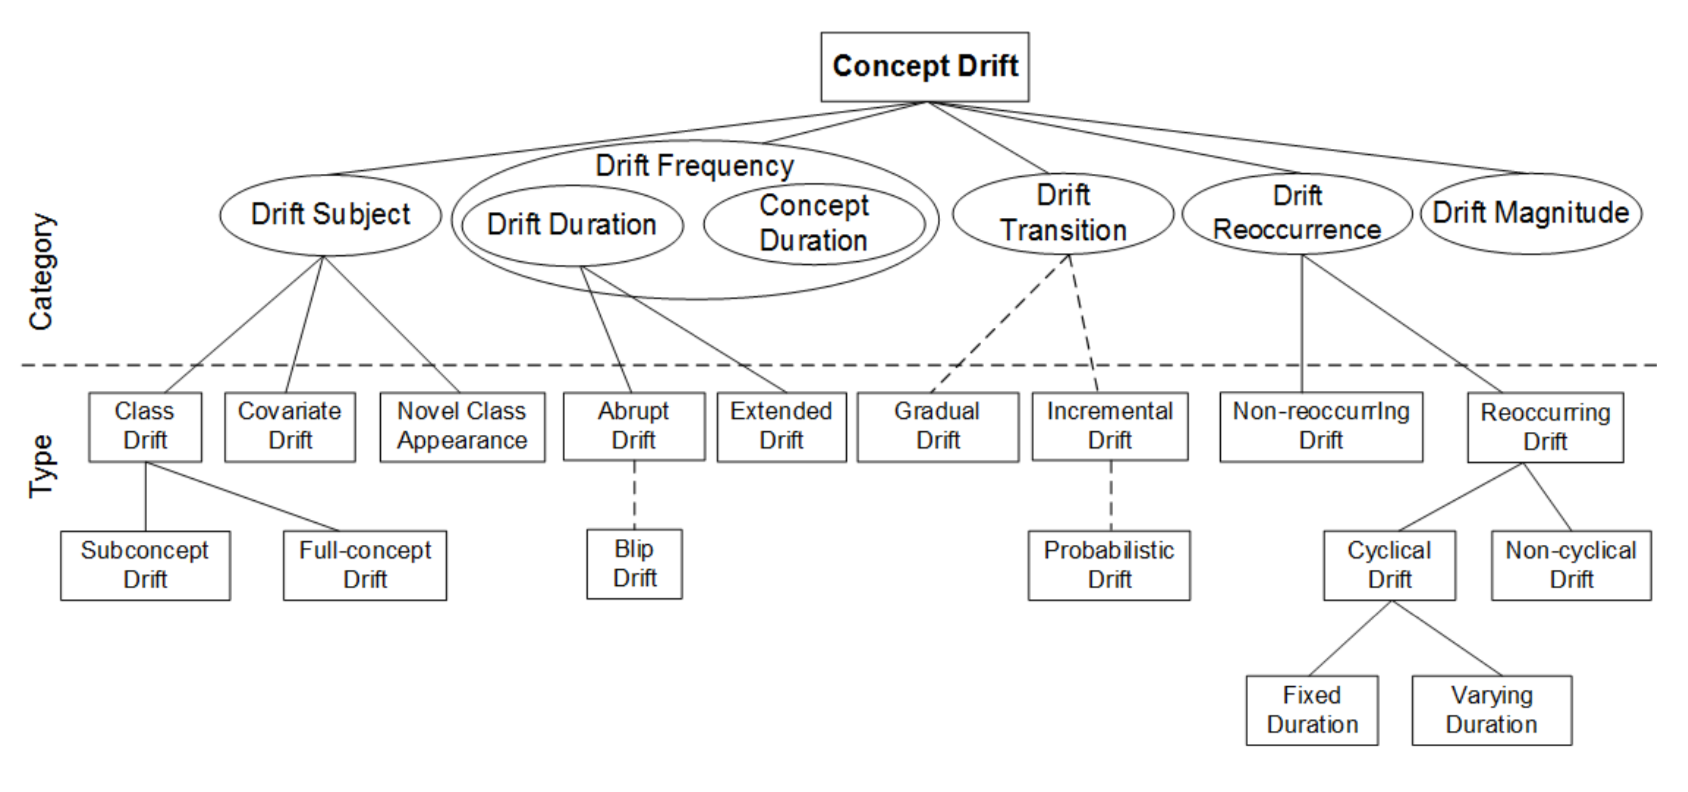
\includegraphics[width=\textwidth]{images/drift_taxonomy.png}
    \caption{Taxonomy of drift types. Solid lines denote mutually exclusive subcategories. Dashed lines denote non-mutually exclusive subcategories. Illustration originally appeared in Webb et al. \cite{characterizing_drift}.}
    \label{fig:drift_taxonomy}
\end{figure}


%-------------------------------------------------------------------
% RELATED WORK
%-------------------------------------------------------------------

\section{Related Work} \label{background:related_work}

There are broadly two approaches to handling concept drift. ``Blind" approaches do not explicitly model drift, instead allowing the model to gradually adapt to the new environment. ``Informed" approaches, instead employ {\bf drift detectors} to explicitly detect when concept drift has occurred so that the model can be retrained on data from the drift point onward \cite{gama_survey}.

A drift detector is an algorithm which predicts whether drift has occurred for a given data stream
\begin{equation}
    D(Z) \approx \begin{cases}
    1 & \text{if drift has occurred on $Z$} \\
    0 & \text{otherwise}
    \end{cases}
\end{equation}
The following are desirable properties for a drift detector:
\begin{itemize}
    % \item A detector should ideally be {\bf transparency} This enables practitioners to both understand the shortcomings of the model and identify when it is going wrong, and also should allow them to trust the system more, given they can actually see its internal mechanisms.
    \item {\bf Adaptiveness} The ability to detect when concept drift has occurred in a short span of time so that model retraining can commence quickly.
    \item {\bf Accuracy} The system should have a low rate of false-positives and false negatives, so that unnecessary training isn't invoked, and necessary training isn't neglected.
    \item {\bf Robustness} The system should be robust to noise.
\end{itemize}

We now present a survey of the field of concept drift detection research.

% \section{Theoretical Results Pertaining to Concept Drift}
% Holembold and Long (1991, 1994) provide an algorithm which is adaptable to drift up to a given extent.
% Kuh , Petsche, and Rivest (1991, 1994) provide an algorithm and theoretical guarantees for a maximum rate of drift. Their approach is based on the PAC framework.

\subsection{Early Algorithms}

The Page-Hinkley Test (pht), also known as CUSUM, introduced the field of change detection, which concept drift detection has grown out of \cite{CUSUM}. This algorithm was proposed in the context of industrial quality control. We imagine testing fixed-size samples of some product from various batches. The number of faulty products from batch $i$ is given by $x_i$. We would like to raise the alarm that the industrial process has gone awry whenever the following condition is met:
\begin{equation}
    \begin{cases}
        x_n > 1 & \text{or} \\
        x_n + x_{n-1} > 2 & \text{or} \\
        \vdots \\
        \sum_{i=0}^k x_{n-i} > k + 1 & \text{for some $k$}
    \end{cases}
\end{equation}
This is equivalent to recording the cumulative sum $S_n = \sum_{i=0}^n x_i$ and raising the alarm whenever
\begin{equation}
    S_n - \min_{i} S_i > h
\end{equation}
for some $h$. In practice, this means we need only keep two registers. First, $S_n$ which accumulates $x_i$, and $S_{min}$, which stores the minimum value of $S_i$ encountered so far.

This equation can easily be adapted to detect significant deviations in both the positive and negative directions. CUSUM may therefore be used to detect change in any real-valued time series. It can also be used to detect changes in a binary-valued series, if the series is processed in batches, as in the motivating example. 

Work on concept drift often describes ad-hoc adaptations of CUSUM to the problem of concept drift detection \cite{barros_comparison}\cite{gama_survey}. These works cite the original paper by Page \cite{CUSUM}, making the author of these variations unclear. I have elected to describe the original form of the algorithm as it is more elegant and theoretically justified than its variations.

The study of concept drift {\it per se} appears to originate with the STAGGER algorithm \cite{STAGGER}. In it's early form, this study was concerned with how ``concepts" - that is, conjunctions of boolean variables such as {\tt bachelor = unmarried AND man} - were ``drifting" over time.  With the introduction of the STAGGER algorithm also came the STAGGER dataset, a synthetic dataset in which instances were classed as positive if they satisfied a certain conjunctive expression. 

The FLORA family of algorithms expanded the study of symbolic concept drift to include recurring concepts and the maintaining of a sliding windows of recent examples \cite{FLORA}. 

Klinkenberg and Joachim subsequently expanded the study of concept drift to real-valued domains \cite{SVM_detection}. Their approach was to train an SVM online, using a sliding window whose size is chosen to minimise generalisation error, which is estimated with the $\zeta\alpha$ estimator. Although this approach was efficient and theoretically well motivated, it was tied specifically to SVMs, and so was not a general solution to the problem of concept drift detection.

\subsection{Drift Detection Method}

Drift detection method (DDM) monitors the error rate of the model. If the error rate changes significantly then this is regarded as an indication of drift having occurred. Classification accuracy is regarded as binary, so the string of correct/incorrect labels by the base learner can be regarded as a sequence of binary independent trials. The error rate is therefore expected to follow a binomial distribution. When the error rate reaches its lowest point $p_{min}$, and its lowest standard deviation $s_{min}$, which is given by $s_i = \sqrt{p(1-p)/i}$. When the error rate is detected to be three standard deviations from the earlier estimate, drift is considered to have occurred and the base model is retrained.

Drift Detection Method (DDM) introduced several ideas which would later become staples of concept drift research. They made the following observations:
\begin{itemize}
    \item By monitoring the residual of the predictions - i.e., the difference between the prediction and true label - rather than something internal to the model, we can treat concept-drift detection as model-agnostic. Specifically, DDM treats the residual as a Bernoulli variable, which takes the value 1 for an incorrect prediction and 0 for a correct prediction.
    \item Under normal conditions of no concept drift, we would normally expect the mean residual to either hold steady or decrease over time. Thus if the mean residual increases, this is indicative of concept drift. Specifically, the authors justified this claim in terms of PAC learning theory. We should therefore keep track of the minimum mean residual so far observed.
    \item We can estimate how unlikely the current observations are under the null hypothesis that no concept drift has occurred. Once the probability of the current observation falls below a certain threshold $W$, a warning is sounded that drift may be occuring and instances start to be recorded in a buffer. When the probability falls below a lower threshold $D$, then drift is regarded to have occurred and the model is retrained on the instances stored in the buffer. If the probability of the current observations returns to a level above the warning threshold, then the buffer is emptied.
\end{itemize}
In DDM, the variable denoting whether or not the classification was correct is a Bernoulli variable, whose probability $p$ of a successful trial (i.e., incorrect classification) can be estimated at time $t$ as $\hat{p}_i$ as the proportion of unsuccessful predicitons so far observed. The standard error around the measurement $\hat{p}_i$ is given by $s_i = \sqrt{p_i(1-P_i)/i}$, and when $p_i+s_i$ reaches its minimum, this will be our lowest probability within a 1-SE confidence interval.

This algorithm is poorly justified. The posterior probability of the rate can be exactly expressed as a beta distribution, so there is no strict need to approximate it with a normal distribution. This approximation will perform poorly when $q$ is close to 0 or 1, and when few data points are available. Furthermore, detecting when the current one-sigma upper bound on the rate exceeds the historically lowest value of the two- or three-sigma upper bound is frankly a silly proxy for detecting when the current rate is larger than its lowest value. One can only obtain a p-value by comparing an upper bound with a lower bound.

However, the more lasting contribution from this paper was to establish a template for drift detectors, with a warning and drift threshold. When the warning threshold is exceeded, all new instances are placed in a buffer. When the drift threshold is exceeded, signal that drift has occurred and train a new model on the contents of the buffer.

RDDM is a variant of DDM with periodic resets to become more reactive to changes in the error-rate. EDDM is another variant, which monitors for changes in the distribution of {\it gaps} between errors, rather than changes in the error rate itself \cite{EDDM}.

\subsection{Sliding Window Approaches}

STEPD essentially approaches concept drift detection by testing the hypothesis ``the error-rate changed $n$ time steps ago for some fixed, and pre-set $n$" at each time step \cite{STEPD}. This is achieved by partitioning the data stream history into 1) a sliding window of the most recent $n$ values, and 2) the preceding values. The statistical test of equal proportions is then used to test whether the rates of the two partitions are significantly different.

FTDD \cite{FTDD}%, FPDD \cite{FPDD}, and FSDD \cite{FSDD} are NOT SURE IF THESE EXIST
~is a variant of STEPD, which uses Fischer's exact test %or the chi-square test 
in place of the test of equal proportions, because the latter is inappropriate for small or imbalanced data. WSTD is another variant, which uses the Wilcoxon rank sum statistical test instead of the test of equal proportions, and additionally limits the size of the second partition \cite{WSTD}.

PL (paired learners) is another sliding window method \cite{PL}. However, rather than testing for differences in error rates of a single model between the two partitions, it instead tests for differences in the error rates of two models. One model, the ``stable learner" is trained online on the entire data stream, and the other, the ``reactive learner" is trained only on the contents of the sliding window. If the proportion of instances in the window that are classified correctly by the reactive learner, but not the stable learner, exceeds some threshold, then drift is indicated.

FHDDM may be considered a hybrid of DDM and sliding window methods \cite{FHDDM}. At each time step the error rate in the sliding window is estimated. If this error rate significantly exceeds its lowest value, then drift is indicated.

\subsection{ADWIN}

A major flaw of the sliding window approaches is that they are brittle with respect to the window size parameter. If the window size is too large then there will be a large delay in the drift detection. If the window is too small then the detector will not be able to detect small drifts over random noise. ADWIN combats this problem by dynamically increasing or decreasing the window size \cite{ADWIN}. The authors explain:
\begin{displayquote}
The idea is simple: whenever two ``large enough" subwindows of $W$ exhibit ``distinct enough" averages, one can conclude that the corresponding expected values are different, and the older portion of the window is dropped. In other words, $W$ is kept as long as possible while the null hypothesis ``$\mu_t$ has remained constant in $W$" is sustainable up to confidence $\delta$.
\end{displayquote}
This involves testing for drift at each time step in the window, which requires a multiple comparisons correction. One of the main advantages of ADWIN is that it provided theoretical guarantees on its false positive and negative rates.

SEQDRIFT \cite{SEQDRIFT} and SEED \cite{SEED} are similar to ADWIN, but they use a different kind of memory management.% I guess. 
SEQDRIFT uses a ``reservoir" and SEED uses ``blocks". %TBH, I don't understand the motivation nor the details of these algorithms.

\subsection{EWMA}

An exponentially weighted moving average (EWMA) is an estimation of a variable $x$, which gives exponentially more weighting to more recent examples:
\begin{equation}
  \hat{x}_t = \lambda \hat{x}_{t-1} + (1-\lambda) x_t
\end{equation}
where $\lambda$ is the decay factor. EWMA is employed in several drift detection methods as it provides a way of estimating the current error rate of the model without knowing how far back in time a drift occurred. When the EWMA estimation of the error rate is significantly larger than the overall mean error rate, then we may conclude drift has occurred. ECDDM is a straightforward application of EWMA to concept drift detection, deriving p-values from a lookup table \cite{ECDDM}. LFR also uses EWMA, although p-values are derived from Monte Carlo estimation \cite{LFR}.

\subsection{HDDM}

The authors cast the drift detection problem as follows. There are $n$ examples $x_1,\dots,x_n$, and a hypothesised drift point $d$. The instances before the drift point are denoted $X=x_1,\dots,x_{d-1}$, and their mean is denoted $\mu_X$. Similarly, those instances after the drift point are denoted $Y=x_d,x_{d+1},\dots,x_n$, and their mean $\mu_Y$. These means are estimated using either the sample average or exponentially weighted average. Depending on which estimator is used, the method is known as HDDM$_A$ or HDDM$_W$. The estimations are denoted $\hat{\mu}_X$ and $\hat{\mu}_Y$, respectively. The authors derive bounds for $P(\hat{\mu}_X+\epsilon < \hat{\mu}_Y|\mu_X \ge \mu_Y)$ and $P(\hat{\mu}_X > \hat{\mu}_Y|\mu_X+\epsilon < \mu_Y)$, thus bounding the false positive and false negative rates, respectively.

This is incorporated into an online drift detection algorithm as follows. At time $t$, the hypothesised drift point is set to $d=t$, and is fixed at this value until enough instances are accumulated to the right of the drift point that either $P(\hat{\mu}_X+\epsilon < \hat{\mu}_Y|\mu_X \ge \mu_Y)$ is statistically insignificant, in which case a drift is signalled, or $P(\mu_X+\epsilon < \mu_Y)$ is statistically insignificant, in which case $d$ is set to the current time step. A major advantage of HDDM is that the derived bounds do not assume that the data stream to be monitored is Bernoulli, so can be used to detect drift on real-valued loss streams.


By constrast, LFR monitors the true negative rate and true positive rate, that is, $P(\hat{y}=i|y=i)$ for $i=0$ and $i=1$ respectively, as well as negative predicted value and positive predicted value, $P(y=i|\hat{y}=i)$ for $i=0$ and $i=1$ respectively. 

% https://www.desmos.com/calculator/mpft6rnqta


% \section{GP Referrals Triage} \label{Background:Medical}

% Etc.

\subsection{Region Drift}

degree of drift DoF
"The proposed method, which can detect different types of drift, is based on processing data chunk by chunk and measuring differences between two consecutive batches, as drift indicator. Differences are calculated by finding nearest neighbour in previous batch of data for each instance in current batch and comparing their corresponding labels.""
The Degree of Drift (dof) processes the data in batches and finds the nearest neighbour of each instance in the current batch in the previous batch. A metric called degree of drift is computed based on this comparison and the differences of labels between nearest neighbour pairs. If the degree of drift changes significantly in one batch, then drift has occurred.

LDD

\subsection{Unbalanced Classes}

ELM

From \cite{DDM_OCI}
\begin{quote}
  First,  most  traditional  methods  detect  drifts based on the drop of overall accuracy or the increase of error made  by  the  learner,  such  as  EDDM  and  DDM.  However, these  measures  are  not  appropriate  for  imbalanced  data  as they  are  sensitive  to  class  imbalance  and  cannot  reflect the  performance  on  the  minority  class  well.  The  minority class  contributes  too  little  to  these  performance  measures compared  to  the  majority  class.  Second,  too  few  examples from the minority classes can make the time arbitrarily long until  the  concept  drift  is  detected,  which  makes  it  difficult to  infer  the  source  of  the  error  for  the  minority  class  –  adrift  or  merely  a  result  of  noise.  Third,  the  minority-class  performance  can  be  very  poor  due  to  the  imbalanced distribution.  It  may  cover  the  effect  of  concept  drift  for detection. Fourth, a class can turn into minority or majority over  time,  so  that  drift  detection  methods  may  need  to  be adapted accordingly. Finally, the performance measures can vary  greatly  with  the  chosen  online  learner.  Any  of  them could be the reason that affects the effectiveness of existing drift detection methods.
\end{quote}


STAGGER was largely focused on a cognitive psychology, rather than practical machine learning perspective.

FLORA used a sliding window. FLORA2 increased or decreased the window size depending on the stability of the data stream. FLORA3 retained previous concepts in memory, and so as to detect recurring concepts.

MDDM looks uses both a sliding window {\it and} geometric or linear weighting, and uses the McDiarmid bound. It detects increases in the weighted error rate in the window.

PerfSim considers all the components of the confusion matrix, and uses the cosine similarity test to detect changes. Drift point candidates are given by assuming the data arrives in batches. CSDD uses the same drift test but uses two fixed-size sliding windows for recent and old data.

The main contribution of CDDM was to take what is in reality a very difficult problem, distill it down to a simple and intuitive formulation, and then offered a terrible solution to the problem as formulated. This naturally stimulated a great deal of follow up work, as other authors could quickly develop an intuition for the problem domain and previous solutions, and come up with improvements on previous these solutions. Plus, there was strong motivation for the problem, and yet a precedent has been set for ignoring the real-world complications which make the problem hard. Scholars interested in starting a new field to accrue massive  ``pioneering work" citations should take note.

This problem formulation is well suited to academic research, as it admits of straightforward notation, experimentation,
However, the formulation often does not fit practical data science applications well.

Another branch of concept drift detection research applies Bayesian modelling to the data stream.

From DDM: Other relevant works are the works of R.Klinkenberg and C.Lanquillon, both of them in information filtering. For instance, Klinkenberg and Renz in [4], in order to detect concept drift, propose monitoring the values of three performance indicators: accuracy, recall and precision over time, and then, comparing it to a confidence interval of standard sample errors for a moving average value (using the last M batches) of each particular indicator.

\subsection{Summary}

With some simplification, we can understand drift detectors as consisting of three components. A drift detection method consists of three components. First there is the method of generating 

\begin{table}[]
    \centering
    \begin{tabular}{|l|l|l|l|}
         \toprule
         Detector & Drift Point Candidates & Statistical Test & Operationalisation  \\
         \midrule
         ADWIN & All & Hoeffding & $D(\yhat=y)$ \\
         CUSUM & - & - & $D(\yhat=y)$ \\
         DDM & Moving Average & - & $D(\yhat=y)$ \\
         EDDM & ? & ? & $D(\yhat=y)$ \\
         EWMA & ? & ? & $D(\yhat=y)$ \\
         FHDDM & ? & ? & $D(\yhat=y)$ \\
         FHDDMS & ? & ? & $D(\yhat=y)$ \\
         HDDM & Window & Hoeffding & $D(\yhat=y)$ \\ 
         MDDM & ? & ? & $D(\yhat=y)$ \\
         PH & ? & ? & $D(\yhat=y)$ \\
         RDDM & ? & ? & $D(\yhat=y)$ \\
         SEED & Blocks & Bernstein & $D(\yhat=y)$ \\ 
         SeqDrift2 & ? & ? & $D(\yhat=y)$ \\
         LFR & Movign Average & Something & $D(\yhat=y|y) \land D(\yhat=y|\yhat)$  \\
         \bottomrule
    \end{tabular}
    \caption{Summary of existing drift detectors}
    \label{tab:drift_detectors}
\end{table}

%-------------------------------------------------------------------
% CONCLUSION
%-------------------------------------------------------------------

\section{Conclusion} \label{background:conclusion}


